208. \begin{figure}[ht!]
\center{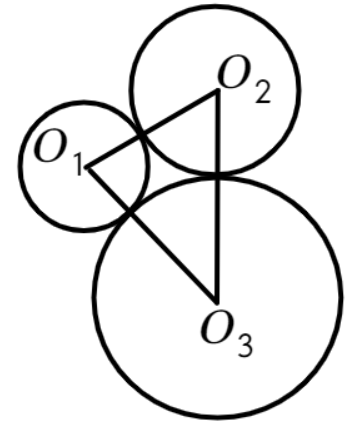
\includegraphics[scale=0.35]{g8-95.png}}
\end{figure}\\
Точки касания окружностей лежат на одной прямой с их центрами, поэтому $O_1O_2=3+7=10,\ O_1O_3=3+10=13,\ O_2O_3=7+10=17,\ p=\cfrac{10+13+17}{2}=20.$ Посчитаем его площадь двумя способами. С одной стороны, по формуле Герона она равна $\sqrt{20\cdot10\cdot7\cdot3}=10\sqrt{42},$ а с другой она равна $rp=20r.$ Значит, $r=10\sqrt{42}:20=\cfrac{\sqrt{42}}{2}.$\\
